% Created 2021-04-09 五 00:31
% Intended LaTeX compiler: xelatex
\documentclass[bigger]{beamer}
\usepackage{graphicx}
\usepackage{grffile}
\usepackage{longtable}
\usepackage{wrapfig}
\usepackage{rotating}
\usepackage[normalem]{ulem}
\usepackage{amsmath}
\usepackage{textcomp}
\usepackage{amssymb}
\usepackage{capt-of}
\usepackage{hyperref}
\usepackage{ctex}
\usetheme{default}
\usecolortheme{}
\usefonttheme{}
\useinnertheme{}
\useoutertheme{}
\author{郑权}
\date{2021-04-05}
\title{解纽数slides}

\hypersetup{
 pdfauthor={郑权},
 pdftitle={解纽数slides},
 pdfkeywords={},
 pdfsubject={},
 pdfcreator={Emacs 28.0.50 (Org mode 9.5)}, 
 pdflang={English}}
\begin{document}

\maketitle
\begin{frame}{Outline}
\tableofcontents
\end{frame}


\begin{frame}[label={sec:org194fc46}]{研究内容}
\begin{block}{Introduction}
\begin{block}{何为纽结?}
\begin{block}{纽结就是\(\mathbb{R}^{3}\) 中的简单闭曲线}
\end{block}
\begin{block}{用拓扑学的语言:}
在拓扑空间\(X\)中,\(X\)的一个子集\(K\)称作是一个纽结,如果\(K \cong S^{2}\)

\begin{center}
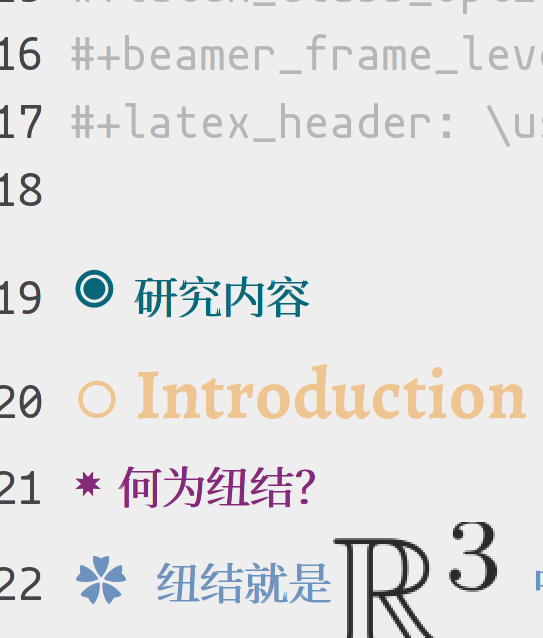
\includegraphics[width=.9\linewidth]{/home/vitalyr/projects/learn/Notebook/org/.attach/86/99c932-5a19-4470-8a7b-d3a6af5fddce/_20210409_003047screenshot.png}
\end{center}
\end{block}
\end{block}

\begin{block}{}
\end{block}
\begin{block}{通俗地说,就说关于三维空间中绳圈的研究。}
\end{block}
\begin{block}{研究什么?}
主要是关于各种拓扑不变量
\end{block}
\end{block}
\end{frame}
\begin{frame}[label={sec:orgaef2a97}]{进展}
\end{frame}
\begin{frame}[label={sec:org1b6900d}]{问题}
\end{frame}
\begin{frame}[label={sec:orgc8a33ab}]{后续计划}
\end{frame}
\begin{frame}[label={sec:orgf3e16e8}]{查阅资料情况}
\href{20210408031644-毕业设计中期答辩slides.org}{毕业设计中期答辩slides}
\end{frame}
\end{document}
